\section{Finally Big Data}

\subsection{Map Reduce Model}

\textbf{How can I scale the transformations to bilions of rows?}

MapReduce is a programming model proposed in a Google paper (2003)to easier multi-node process parallelization:

\begin{itemize}
	\item Users specify a map function that processes a key/value pair to generate a set of intermediate key/value pairs, and a reduce function that merges all intermediate values associated with the same intermediate key
	\item Programs written in this functional style are automatically parallelized and executed on a large cluster of commodity machines
	\item Inputs and operations over inputs are processed in parallel by different machines using a partitioning function (e.g., hash(key) mod R)
\end{itemize}  

\begin{center}
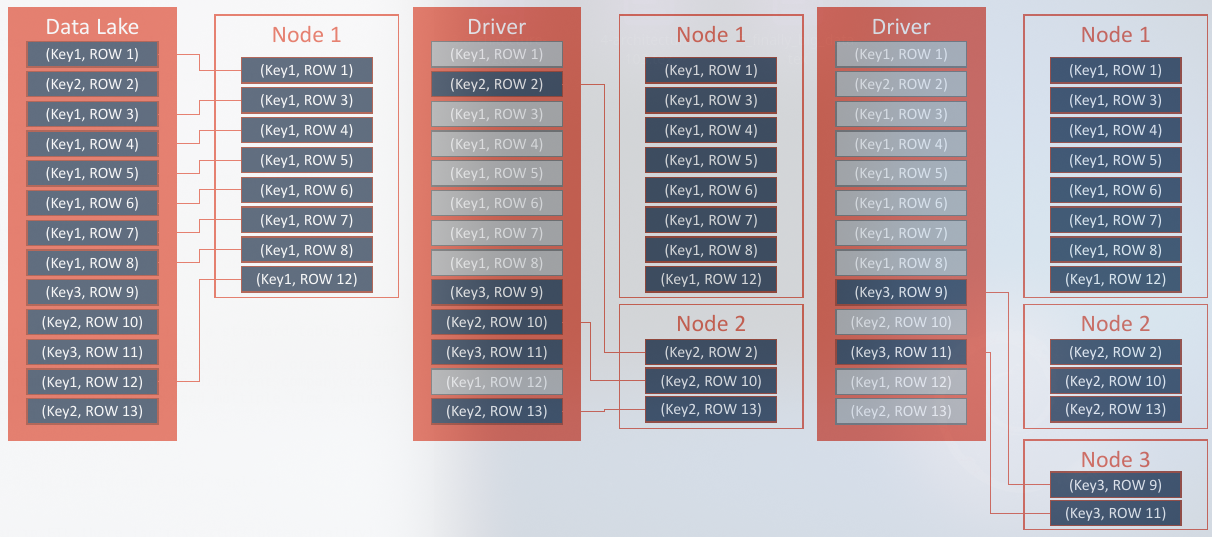
\includegraphics[scale=0.5]{51-map-reduce-model-1}
\end{center}

\begin{center}
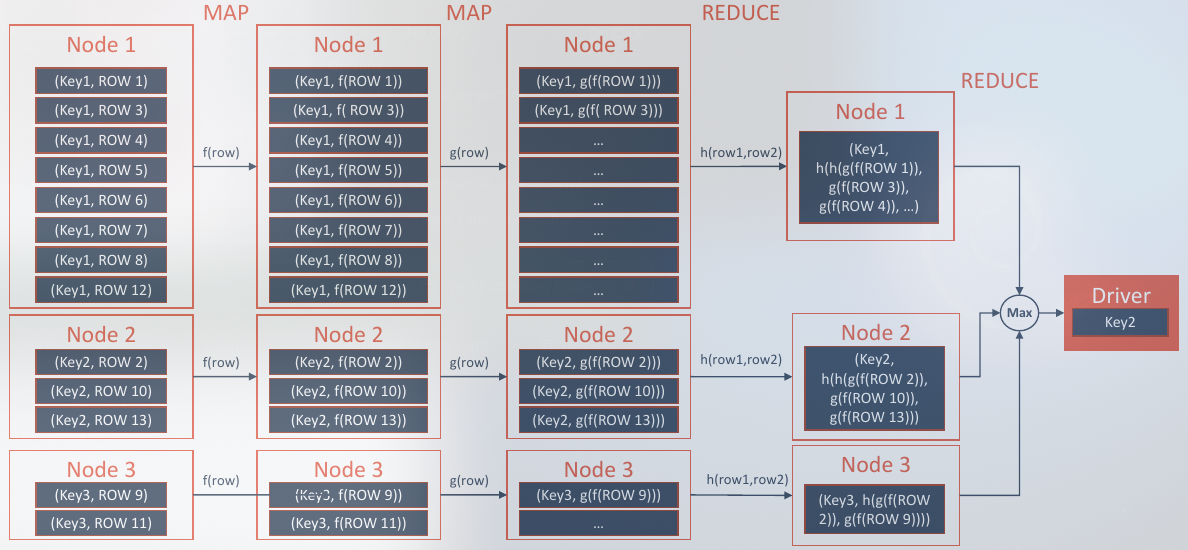
\includegraphics[scale=0.5]{51-map-reduce-model-2}
\end{center}

\subsection{Apache Hadoop}

\textbf{Distributed Parallel Frameworks}

\textbf{How to process data at scale}

\begin{itemize}
	\item Framework of -mostly- \textbf{open source components} built to facilitate the development of multi-node services written in Java
	\item Based on the assumption \textbf{hardware can fail}, several high reliability strategies are used inside Hadoop
	\item Three main components
	- \textbf{STORAGE} - Hadoop Distributed File System Storage (HDFS)
	- \textbf{RESOURCE MANAGEMENT} - Hadoop YARN
	- \textbf{PARALLEL COMPUTATION} - Hadoop MapReduce (implementation of Map Reduce pattern)
	\item Any Hadoop component should be location aware (name of the network switch where each node is) and should share it to the system to distribute data and computation
\end{itemize}

\subsection{Apache Architecture}

\begin{center}
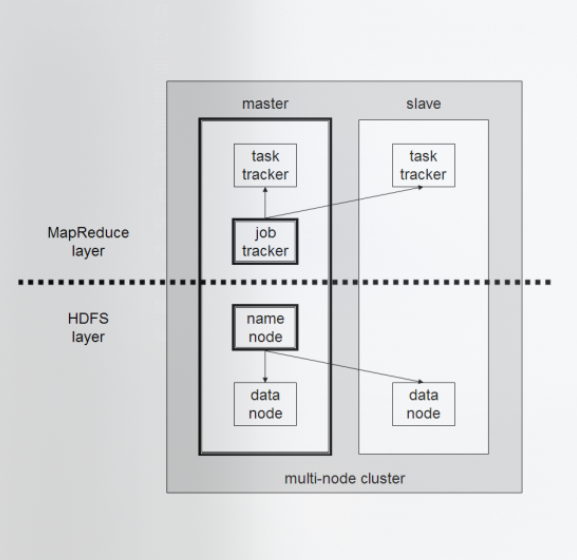
\includegraphics[scale=0.5]{52-hadoop-architecture-1}
\end{center}

\begin{itemize}
	\item \textbf{Job Tracker}
	- service that decide where a given task should be executed (ideally the nodes that have the data, or closer one)
	\item \textbf{Task Tracker}
	- a nde in the cluster that accepts tasks from a JobTracker. It expose a finite number of slots that represents its capability of run parallel tasks. Each task is executed on a spawned JVM. It also sends an heartbeat to the Job Tracker every minute to reassure it is still alive
\end{itemize}

\begin{itemize}
	\item \textbf{NameNode}
	- It keeps the directory tree of all files in the file system, and tracks where across the cluster the file data is kept. It does not store the data of these files itself. It is the Single Point of Failure of an Hadoop application. It routes request between application and DataNode
	\item \textbf{Backup NameNode}
	- Still under development to give to Hadoop High Availability
	\item \textbf{DataNode}
	- Stores data. DataNodes work with each other to replicate data. DataNode with data to process should be deployed on the same machine where TaskTracker is running
\end{itemize}

\begin{itemize}
	\item \textbf{Master Node}
	- Made by a Job Tracker, Task Traker, NameNode, and DataNode
	\item \textbf{Worker Node}
	- Made by a DataNode and TaskTracker
\end{itemize}


\subsection{Apache Sequence}

\begin{center}
\includegraphics[scale=0.5]{52-hadoop-architecture-sequence}
\end{center}

\begin{itemize}
	\item Application submits an asyncronous job to the Job Tracker, then it can start polling the Job Tracker for job status
	\item Job Tracker gets data locations in the Name Node registry
	\item Job Tracker identifies the set of Task Trackers with available slots nearest to Data Nodes
	\item The JobTracker submits the work to the chosen Task Trackes
	\item ob Tracker starts to monitor Task Trackers heartbeat: If they do not submit heartbeat signals often enough, it presumes they failed and work is scheduled on a different Task Tracker.
	\item When each Task Tracker completes the task, it notify the Job Tracker the final status. If it failed, the Job Tracker can:
	1. resubmit the job elsewhere
	2. mark that specific record as to-skip
	3. blacklist the task traker as unreliable
\end{itemize}

